\section{Experiments report}
\label{sec:exp}

In order to evaluate RAOES, we conducted experiments focusing on different aspects. 
Our research questions are as followings:
\begin{description}[\footnotesize]
	\item[\tb{RQ1}] %A state machine \ttt{sm} is used for generating the front-end code. The latter is reversed engineered to produce another state machine \ttt{sm'}. Are \ttt{sm} and \ttt{sm'} identical? In other words: 
	Whether the front-end code generated from a model with USMs can be used for reconstructing the original model. This question is related to the \ti{GETPUT} law defined in \cite{foster_combinators_2007}.
	
	\item[\tb{RQ2}] The back-end code is used for compilation. 
	Does the runtime execution of the back-end code is semantic-conformant to Precise Semantics for UML State Machines (PSSM)? 
	
	\item[\tb{RQ3}] Runtime performance and memory usage is undoubtedly critical in real-time and embedded systems. Particularly, in event-driven systems, the performance is measured by event processing speed. Does code generated by the presented approach outperform existing approaches and use less memory?
\end{description} 

In the followings, Subsections \ref{subsec:exp1}, \ref{subsec:exp2}, and \ref{subsec:exp3} report the experimental results for RQ1, RQ2, and RQ3, respectively.

\begin{figure}
	\centering
	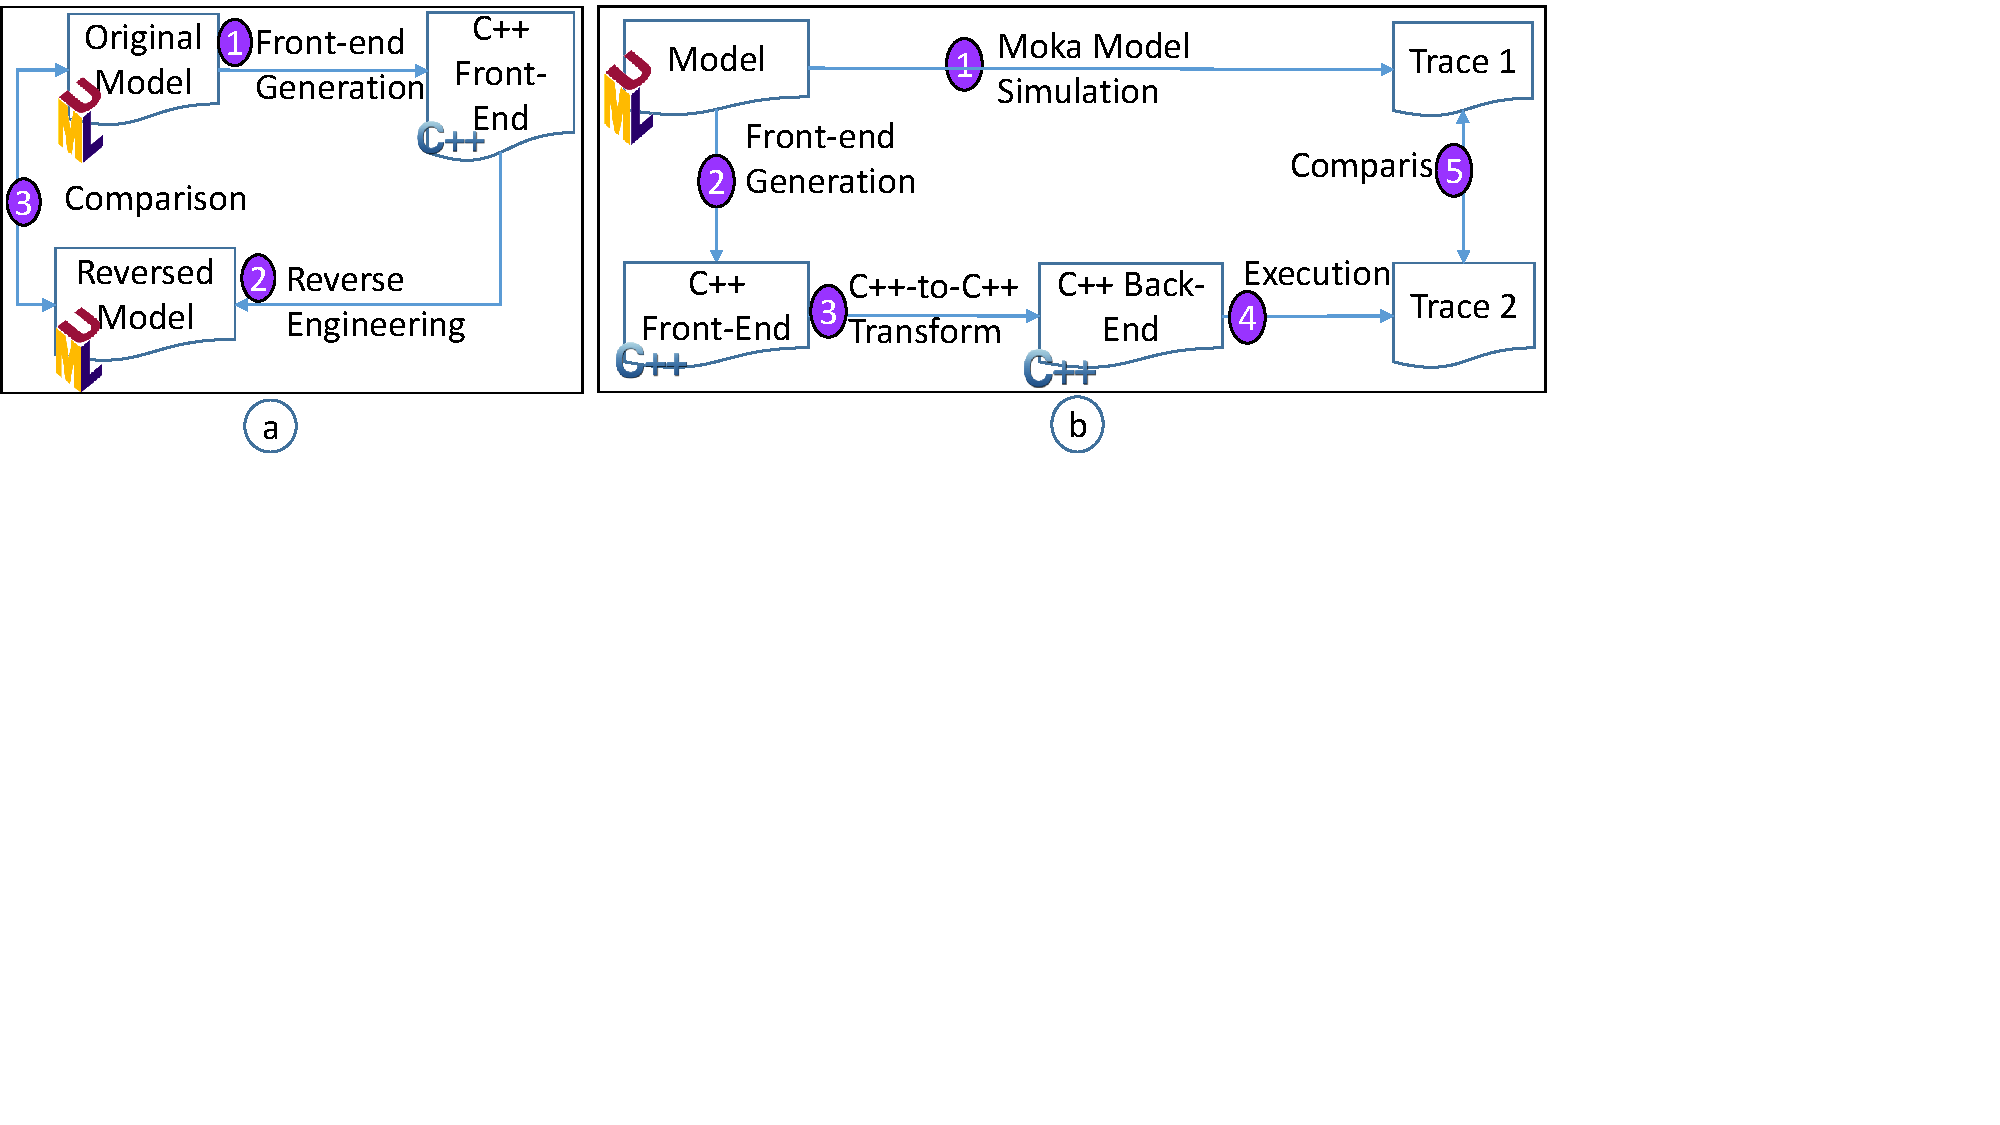
\includegraphics[clip, trim=0cm 11.4cm 7.65cm 0cm, width=\columnwidth]{figures/rq1-2evaluation}
	\caption{Evaluation methodology to answer RQ1 (a) and RQ2 (b)} 
	\label{fig:rq1-2evaluation}
\end{figure}

%\tb{RQ3}: RTE allows developers to freely move between and modify model and code. Specifically, in software development projects, some traditional programmers might want to practice with code in a traditional way and some MDE developers may prefer working with models. What is the development/maintenance cost comparison between the two practices by comparing the number of steps needed to do equivalent actions?

%This section reports our experiments targeting the three questions. Two types of experiments are conducted and presented in Subsections \ref{subsec:exp1} and \ref{subsec:exp2}, respectively. 



\begin{comment}
\begin{figure}
\centering
\includegraphics[clip, trim=5.5cm 19cm 5.5cm 6cm, width=0.3\textwidth]{figures/strategy1}
\caption{Evaluation methodology to answer RQ1} 
\label{fig:strategy1}
\end{figure}

\begin{figure}
\centering
\includegraphics[clip, trim=4.5cm 16.5cm 5.5cm 6.5cm, width=0.3\textwidth]{figures/strategy2}
\caption{Evaluation methodology to answer RQ2} 
\label{fig:strategy2}
\end{figure}
\end{comment}

%Furthermore, in software development projects, some traditional programmers might want to practice with code in a traditional way and some MDE developers may prefer working with models. Therefore, it is necessary to compare the development/maintenance cost between the two practices by comparing the number of steps needed to do the same action. 


\subsection{Reversing generated code}
\label{subsec:exp1}
\tb{RQ1}: A state machine \ttt{sm} is used for generating the front-end code. The latter is reversed engineered to produce another state machine \ttt{sm'}. Are \ttt{sm} and \ttt{sm'} identical? In other words: whether the front-end code generated from USMs model can be used for reconstructing the original model. This question is related to the \ti{GETPUT} law defined in \cite{foster_combinators_2007}.

\begin{figure}
	\centering
	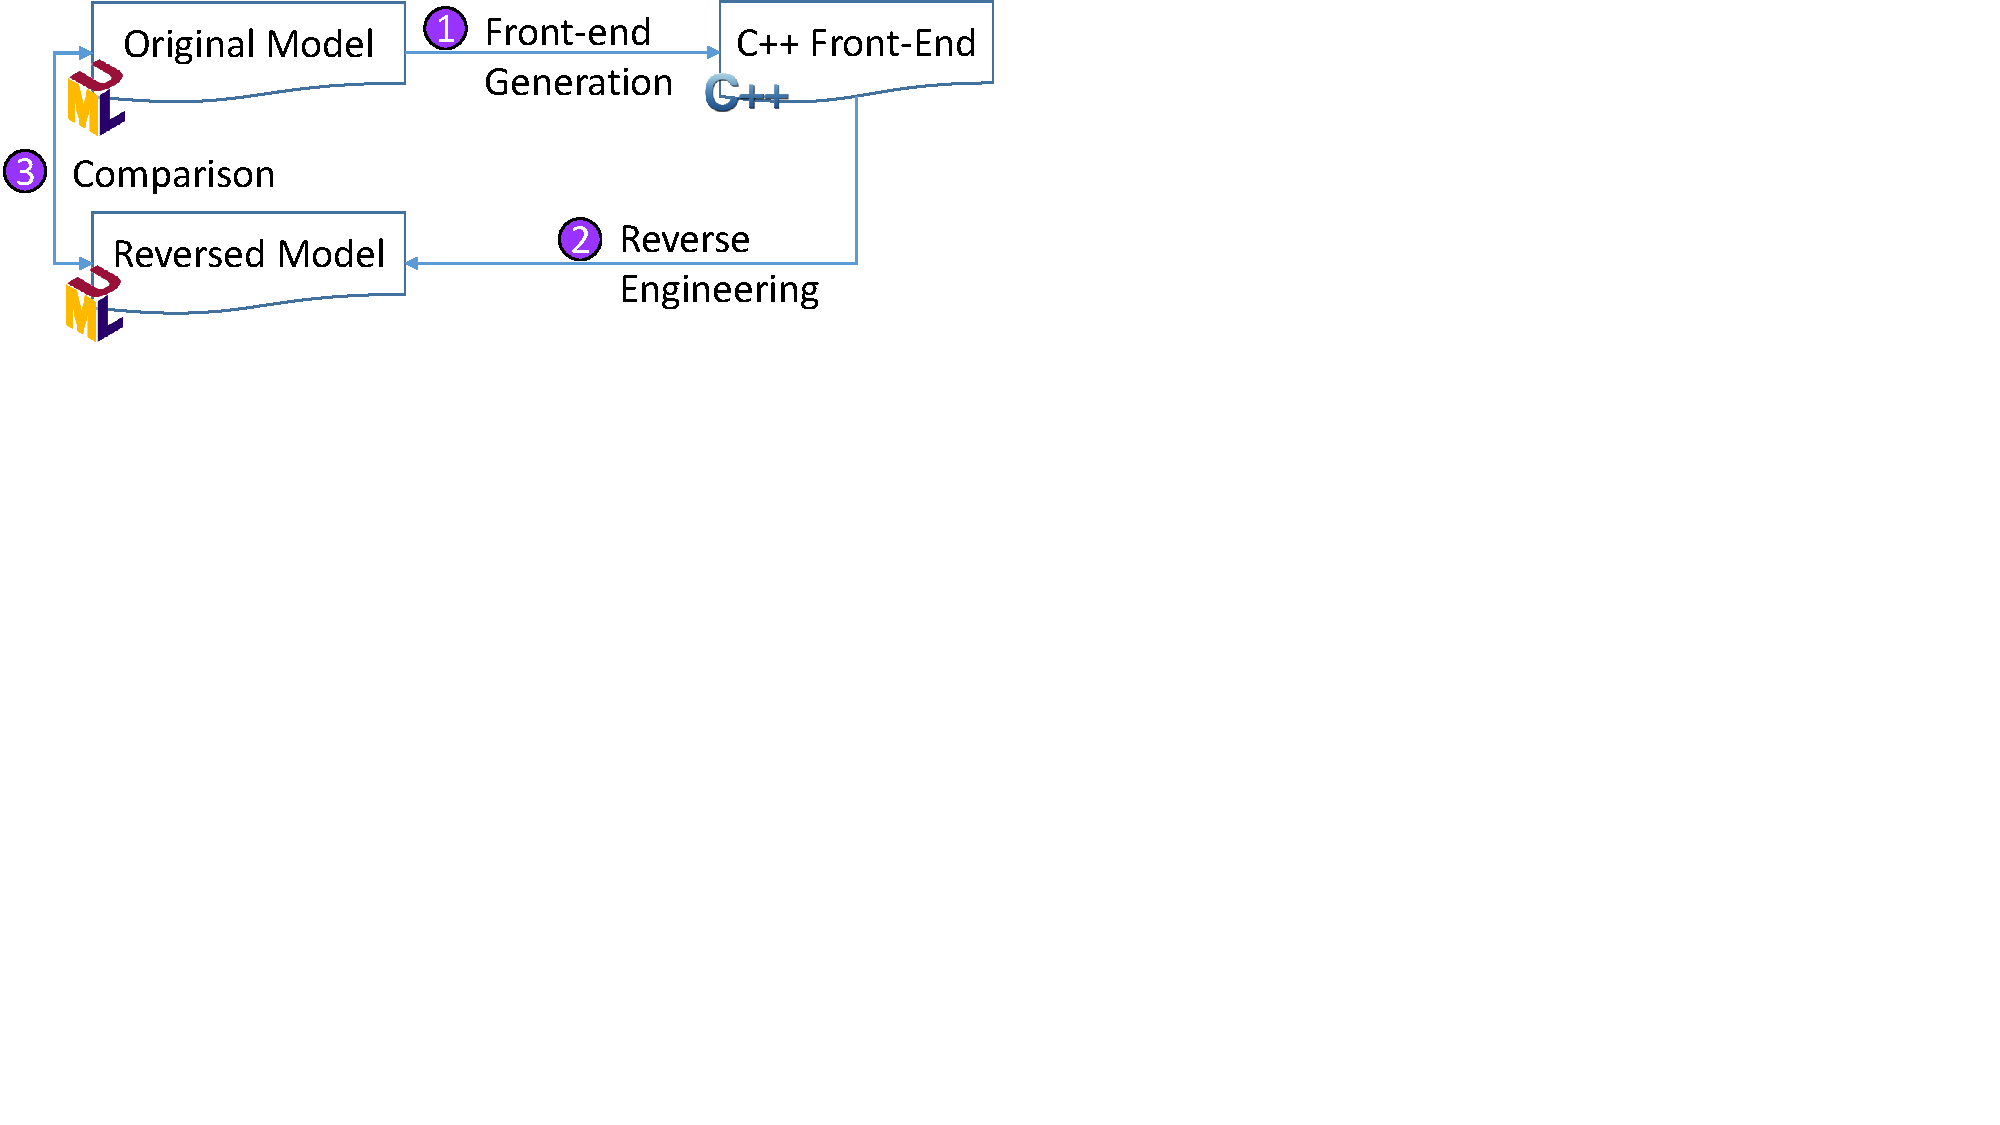
\includegraphics[clip, trim=0cm 13.1cm 16.2cm 0cm, width=\columnwidth]{figures/rteevaluation}
	\caption{Evaluation methodology to answer RQ1} 
	\label{fig:EvaluationStrategyBoth}
\end{figure}

%This experiment is targeting \tb{RQ1}. 
Fig. \ref{fig:EvaluationStrategyBoth} shows the experimental methodology to answer \tb{RQ1}. 
The procedure for this experiment, for each original UML model containing a state machine, consists of 3 steps: 
\begin{description}
	\item[Step 1] \ttt{C++ front-end code} is generated from an \ttt{original model}.
	
	\item[Step 2] The \ttt{C++ front-end code} is reverse engineered to a \ttt{reversed model}
	
	\item[Step 3] The \ttt{reversed model} is then compared to the \ttt{original model}.
\end{description}

%(1) C++ front-end code is generated from an \tb{original model}, (2) the generated code is reverse engineered to a \tb{reversed model}, and (3) the the is then compared to the \tb{original state machine}.% by using information of USM such as the numbers of states and transitions. 

Random models are automatically generated by a configurable model generator. 
The latter can generate a desired average number of vertexes, transitions, and events. 
For each model, a context class and its behavior described by a USM are generated. 
Each USM contains 80 states including atomic and composite states, more than 234 transitions. 
The number of lines of generated C++ code for each machine is around 13500. Names of the generated states are different. 
An initial pseudo state and a final state are generated for each composite state and containing state machine. 
Other elements such as call events, time events, transition/entry/exit actions and guards are generated with a desired configuration. 
For each generated call event, an operation is generated in the context class which is also generated. 
The duration is generated for each time event. 

\begin{comment}
\begin{table}
\centering
\caption{Set-up information for model generation}
\label{table:setup}
\begin{tabular}{|l|l|}
\hline
\rowcolor{Gray}
Description                                     & Value            \\ \hline
%Number of generated states                      & 80               \\ \hline
%Number of generated transitions                 & \textgreater 234 \\ \hline
Probability of having an event for transition   & 0.8              \\ \hline
Probability of having CallEvent for transition  & 0.7              \\ \hline
Probability of having an entry/exit action for state & 0.7              \\ \hline
Probability of having a transition action and guard       & 0.7              \\ \hline
\end{tabular}
\end{table}
\end{comment}

%The set up information for the USM generation is shown in Table \ref{table:setup}. 

\begin{table}
\centering
\caption{Three of model results of generation and reverse: Abbreviations are atomic states (AS), composite states (CS), transitions (T), call events (CE), time events (TE)}
\label{table:law1-resultat}
\begin{tabular}{|l|l|l|l|l|l|l|}
\hline
\rowcolor{Gray}
Test ID & AS & CS & T & CE & TE & Is reverse correct? \\ \hline
1       & 47 & 33 & 234 & 145 & 40 & Yes                 \\ \hline
2       & 42 & 38 & 239 & 145 & 36 & Yes                 \\ \hline
%3       & 43 & 37 & 238 & Yes                 \\ \hline
..      & .. & .. & .. & .. & .. & Yes                 \\ \hline
300       & 41 & 39 &240 & 142 & 37 & Yes                 \\ \hline
\end{tabular}
\end{table}
 
 
\begin{comment}
\begin{table*}[]
\centering
\caption{MODEL RESULTS OF GENERATION AND REVERSE}
\label{table:law1-resultat}
\begin{tabular}{|l|l|l|l|l|l|l|l|l|l|l|l|l|l|}
\hline
\rowcolor{Gray}
Test ID & AS & CS & D  & T   & EA & ExA & TA  & CE  & TE & G   & I  &    & Is reverse correct? \\ \hline
1       & 47 & 33 & 8  & 234 & 53 & 50  & 149 & 145 & 40 & 147 & 34 & 25 & Yes                 \\ \hline
2       & 42 & 38 & 8  & 239 & 52 & 59  & 165 & 145 & 36 & 133 & 39 & 31 & Yes                 \\ \hline
3       & 43 & 37 & 7  & 238 & 54 & 59  & 159 & 141 & 34 & 145 & 38 & 28 & Yes                 \\ \hline
..      & .. & .. & .. & ..  & .. & ..  & ..  & ..  & .. & ..  & .. & .. & Yes                 \\ \hline
300       & 41 & 39 & 10 & 240 & 56 & 55  & 165 & 142 & 37 & 151 & 40 & 33 & Yes                 \\ \hline
\end{tabular}
\end{table*}
\end{comment}

%Table  \ref{table:law1-resultat} shows the number of each type of elements in the randomly generated model, including the comparison results, for 3 of the 200 models created by the generator. We limited ourselves to 200 models for practical reasons

Table \ref{table:law1-resultat} shows the number of several types of elements in the generated models, including the comparison results, for 3 of the 300 models created by the generator. We limited ourselves to 300 models for practical reasons. No differences were found during model comparison. The results of this experiment show that the proposed approach and the implementation can successfully do code generation from state machines and reverse. 

%\input{sections/changepropagation}

%\input{sections/timecomplexity}

%
\subsection{Semantic conformance of runtime execution}
\label{subsec:exp2}
\paragraph{Bisimulation for semantic-conformance}
To evaluate the semantic conformance of runtime execution of generated code, we use a set of examples provided by Moka \cite{moka}. Moka is a model execution engine offering Precise Semantics of UML Composite Structures \cite{OMG2015}. Fig. \ref{fig:semanticconformance} shows our method. We first use our code generator to generate code (Step (1)) from the Moka example set. Step (2) simulates the examples by using Moka to extract the sequence (\ti{SimTraces}) of observed traces including executed actions. The sequence (\ti{RTTraces}) of traces is also obtained by the runtime execution of the code generated from the same state machine in a Step (3). The generated code is semantic-conformant if the sequences of traces are the same for both of the state machine and generated code \cite{Blech2005}. The current version of Moka does not support simulation for \ti{TimeEvent} and history pseudo states, we therefore leave experiments for \ti{TimeEvent} as future work.

For example, Fig. \ref{fig:autotransition} (a) shows a USM example with triggerless transitions (\ti{autotransitions}) \ti{T3}. 
The USM contains two states, \ti{Waiting}, which is the initial state, and \ti{Incrementing}, which increases an integer number from 0 to 5 by using the effect of \ti{T3}. The latter also has a guard checking whether the number is less than 5.
The increase is executed after the USM receives an event named \ti{start} to transition the initial state \ti{Waiting} to \ti{Incrementing}. 
Suppose that executions of the effects of \ti{T3} and \ti{T4} produce traces \ti{<T3>} and \ti{<T4>} (by using MOKA, e.g.), respectively. 
Due to the guard of \ti{T3}, the effect of \ti{T3} is executed five times followed by an execution of the effect of \ti{T4}.
After the completion of the USM, the obtained sequence of traces
is \ti{<T3><T3><T3><T3><T3><T4>} (since the \ti{Incrementing} state does not have an \ti{entry}, \ti{exit}, or a \ti{doActivity}, only the transition effect \ti{T3} produces traces). 
The sequence \ti{RTTraces} obtained by the runtime execution %of the code generated from this USM 
must be equivalent. 
\ti{RTTraces} is obtained by simply printing logging information for each action (effect).

Within our scope as previously defined 30 examples of the Moka example set are tested. \ti{SimTraces} and \ti{RTTraces} for each case are the same. 
This indicates that, within our study scope, the runtime execution of code generated by our generator can produce traces semantically equivalent to those obtained via simulation. 


After experimenting with our code generator, we compare our results to the observed traces obtained by executing code generated 
%by IBM Rhapsody \cite{ibm_rhapsody} and 
Umple \cite{Badreddin2014}. 
We find that the obtained traces in case of 
%IBM Rhapsody and 
Umple are not UML-compliant in triggerless transitions and some cases of event processing.
Specifically, for the example in Fig. \ref{fig:autotransition} (a), 
code generated by Umple only produces \ti{<T3>} as the trace sequence. 
Umple does not support events which are accepted by sub-states and the corresponding composite state as in Fig. \ref{fig:autotransition} (b) in which both \ti{S1} and \ti{S21} accept the event \ti{Continue}.
%Rhapsody does not support self-triggerless transitions as in Fig. \ref{fig:autotransition} and its support for processing events is not totally semantically correct. 
As the processing event example in Fig. \ref{fig:autotransition} (b), assuming that there is an event \ti{Continue} incoming to the state machine which has a current configuration \ti{(S1, S21)} as current active states. While, according to the UML specification, the incoming event should be processed by the inner states of the active composite/concurrent state if the inner states accept it, otherwise the parent state does. Therefore, the next configuration should be \ti{(S1, final state)} and the \ti{T22Effect} effect of the transition \ti{T22} should be executed. %But in case of Rhapsody the next configuration is \ti{End}.   


\begin{figure}
\centering
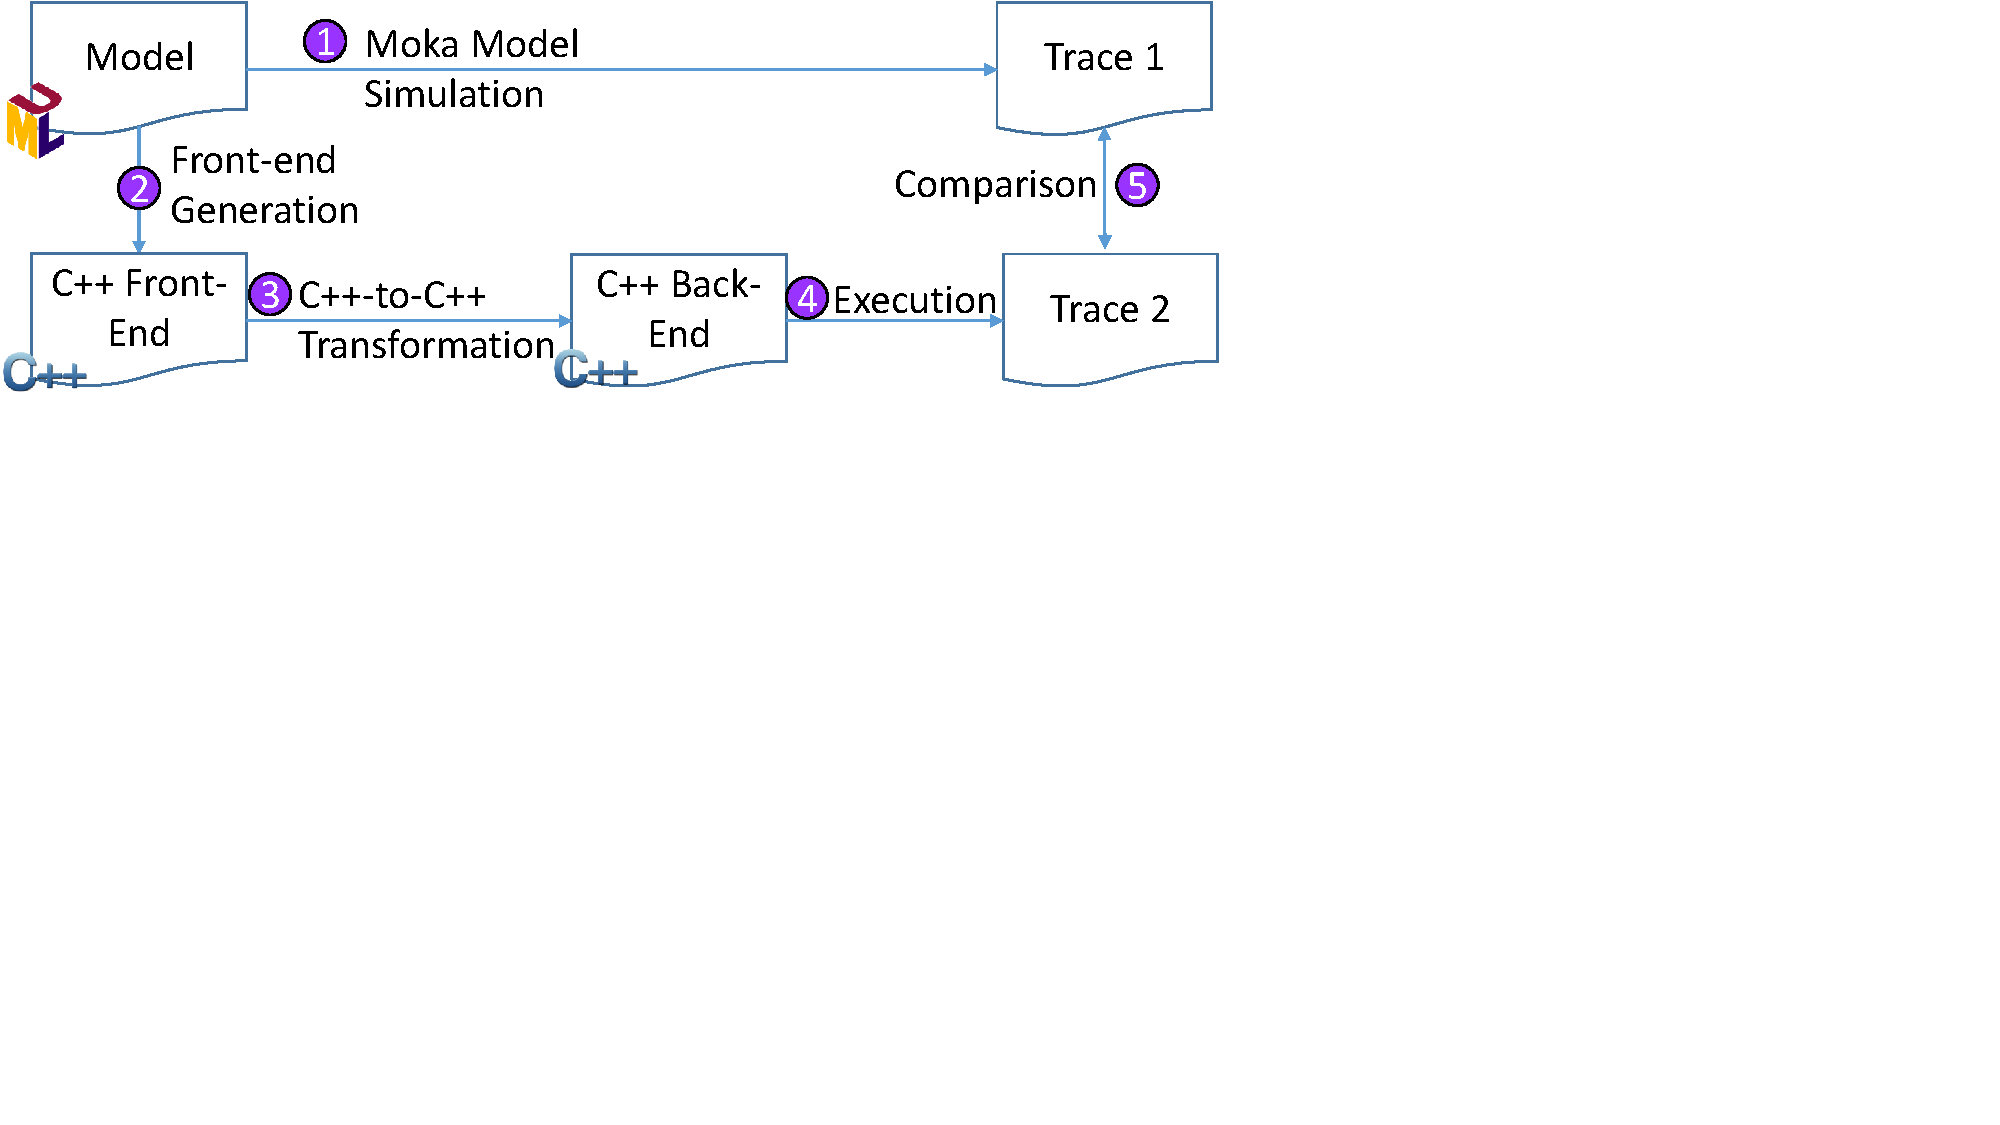
\includegraphics[clip, trim=0.2cm 8.6cm 19.4cm 6.9cm, width=0.8\columnwidth]{figures/semanticconformance.pdf}
\caption{Semantic conformance evaluation methodology} 
\label{fig:semanticconformance}
\end{figure}

\begin{figure}
\centering
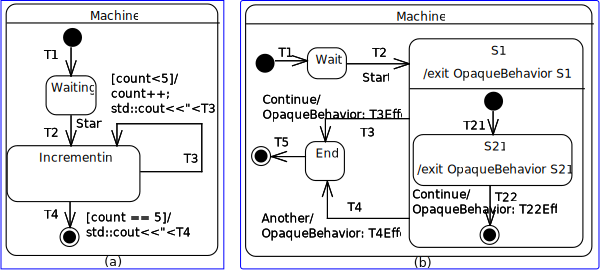
\includegraphics[clip, trim=0cm 0cm 0cm 0cm, width=\columnwidth]{figures/Deferred004Revised}
\caption{Self-triggerless transition and event processing example} 
\label{fig:autotransition}
\end{figure}



\begin{comment}
\begin{figure}
\centering
\includegraphics[clip, trim=0.25cm 0.25cm 0.25cm 0.25cm, width=0.9\columnwidth]{figures/Deferred004}
\caption{Event processing example} 
\label{fig:Deferred}
\end{figure}


\begin{figure*}
\centering
\includegraphics[width=1.5\columnwidth]{figures/ex}
\caption{Self-triggerless transition (a) and event processing (b) examples} 
\label{fig:ex}
\end{figure*}
\end{comment}

\paragraph{Finite state machine}
In addition to the experiment using MOKA, we evaluate the semantic-conformance by using deterministic finite state machines (FSMs). The latter is a mathematical model of computation and also a simplified version of UML state machine. In this experiment, we use FSMs for recognizing input symbols. Each FSM contains many atomic states. The active state of the FSM can be changed following the acceptance of an input symbol. Fig. \ref{fig:fsm} shows our method to experiment. For each FSM, we create an equivalent USM. Each input symbol of the FSM is considered as an event of the USM. We use the FSM simulator in \cite{fsmsim} to generate and simulate FSMs. For each FSM, a list of observed states is recorded as output (\ti{out1}) of the simulation for each symbol list. The latter is also the input of the generated code runtime execution of the equivalent USM which produces an output \ti{out2}. We then compare \ti{out1} and \ti{out2}.

We limit the number of FSMs to 20 and the number of symbol list for each FSM to 30 for practical concerns. 600 sequences of states obtained by the simulation and a same number of sequences taken by the runtime execution are respectively compared and found being equal. This results that our code generation approach can produce semantic-conformant code in case of FSM.

\begin{figure}
	\centering
	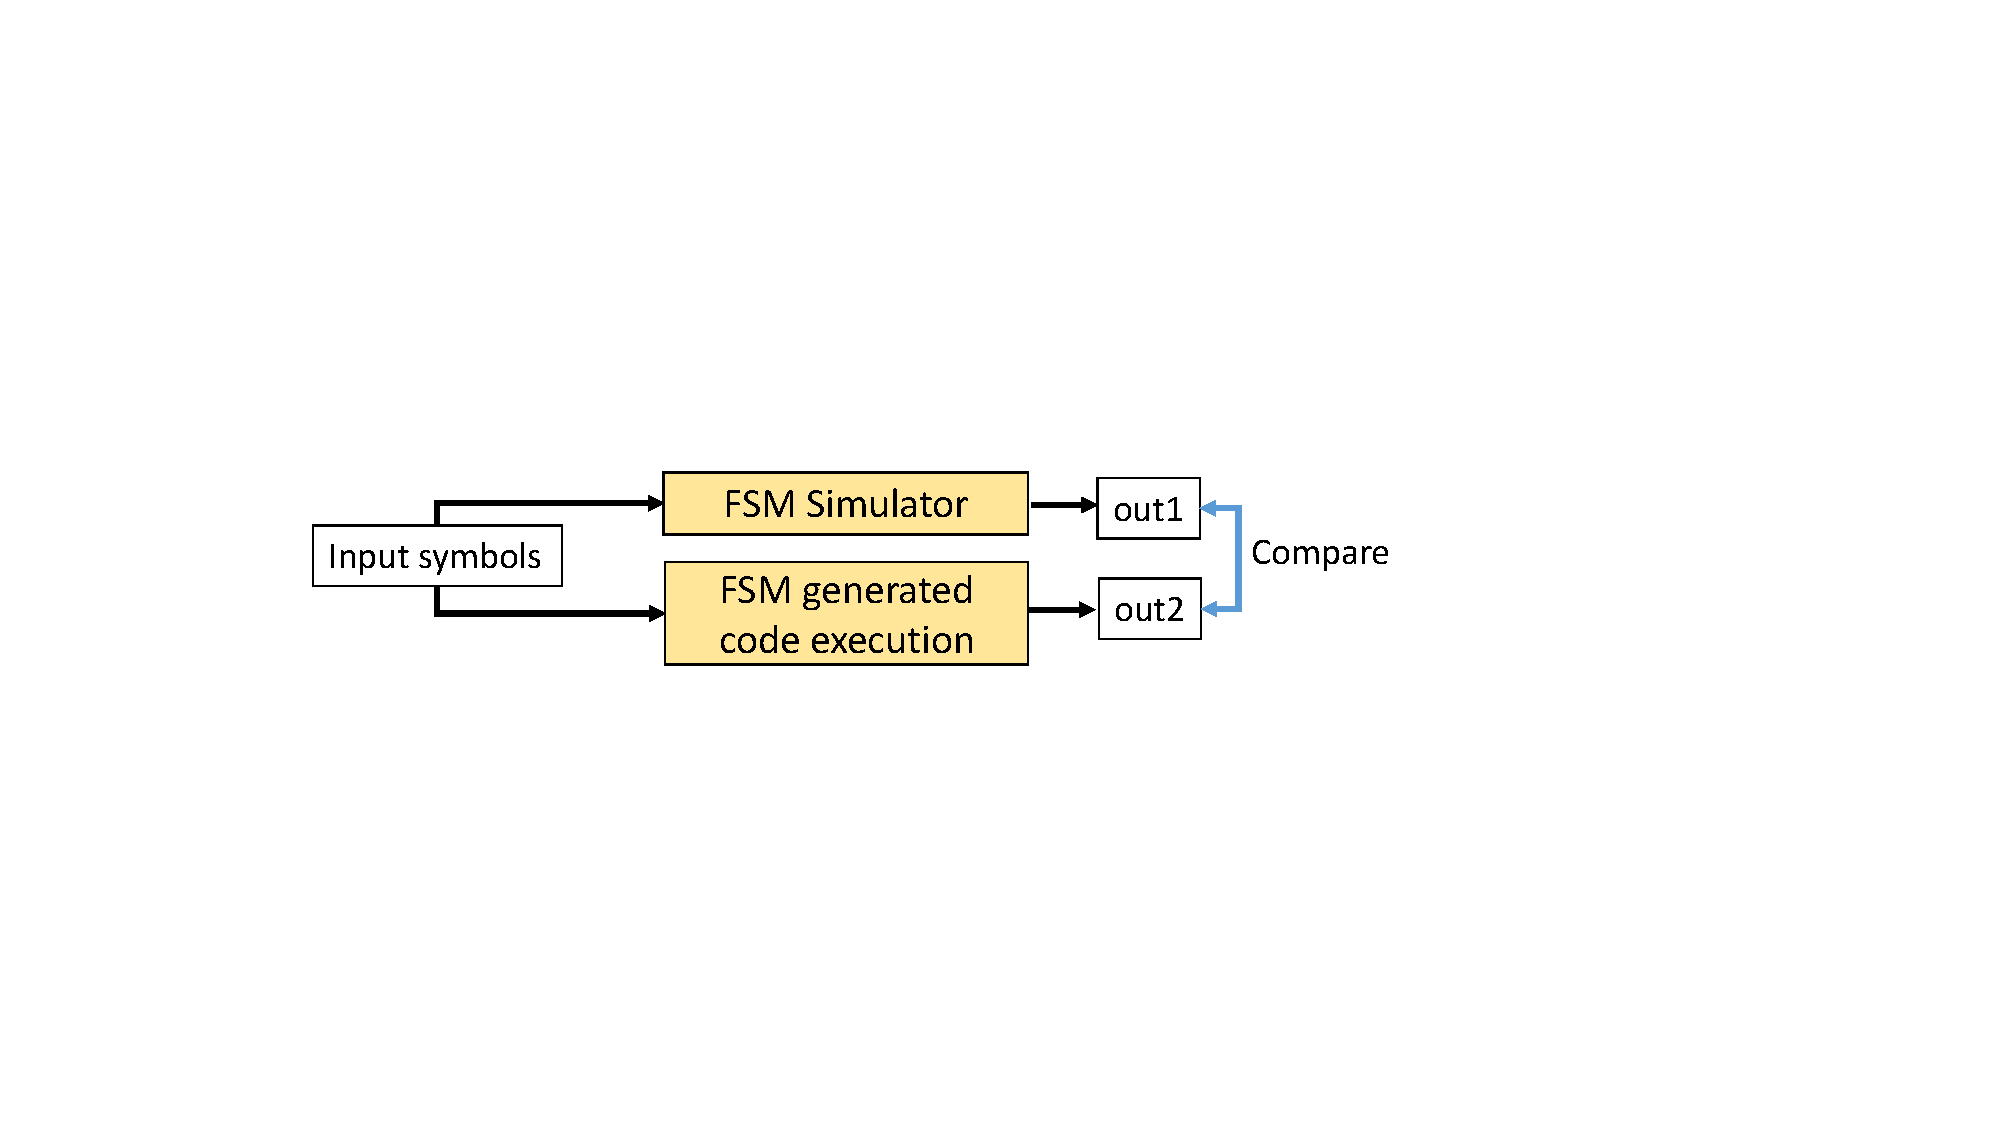
\includegraphics[clip, trim=4.5cm 7.6cm 10.25cm 8.0cm, width=0.85\columnwidth]{figures/fsm}
	\caption{FSM experiment method} 
	\label{fig:fsm}
\end{figure}


%\paragraph{Comparison with IBM Rhapsody}

%\input{sections/developmentcost}

%The approach is implemented as part of the Papyrus Designer tool \cite{qompass} and an extension \tb{PSM} of Papyrus \cite{cea-list_papyrus_????}. This section reports our experiments with \tb{PSM} on the semantic-conformance (Subsection \ref{subsec:exp1}) and efficiency (Subsection \ref{subsec:exp2}) of generated code.

\subsection{Semantic conformance of runtime execution}
\label{subsec:exp2}
%\noindent
%\tb{RQ2:} \ti{The back-end code is used for compilation. Does the runtime execution of the back-end code is semantic-conformant to Precise Semantics for UML State Machines (PSSM)?}.

%\paragraph{Bisimulation for semantic-conformance}
To evaluate the semantic conformance of runtime execution of the back-end code for \tb{RQ2}, we use a set of USM examples provided by \ttt{Moka} \cite{moka}. 
The latter is a model execution engine offering PSSM. 
Fig. \ref{fig:rq1-2evaluation} (b) shows our method, which consists of the following steps:


\begin{description}[\footnotesize]
	\item[Step 1] For a \ttt{model} from the Moka example set, we simulate its execution by using Moka to extract a sequence of traces \ttt{Trace 1}.
	
	\item[Step 2] A \ttt{C++ front-end} code is generated from the \ttt{model} using the front-end generator implemented in Section \ref{subsubsec:gen}.
	
	\item[Step 3] The \ttt{C++ front-end} is used as input for generating a \ttt{C++ back-end} code using the source-to-source transformation.
	
	\item[Step 4] The \ttt{C++ back-end} is compiled for execution to obtain a sequence of traces \ttt{Trace 2}.
	
	\item[Step 5] \ttt{Trace 1} and \ttt{Trace 2} are compared.  
\end{description}

The \ttt{C++ back-end} is semantics-conformant if \ttt{Trace 1} and \ttt{Trace 2} are the same.

%We first use our code generator to generate code (Step (1)) from the Moka example set. Step (2) simulates the examples by using Moka to extract the sequence (\ti{Traces 1}) of observed traces including executed actions. The sequence (\ti{Traces 2}) of traces is obtained by the runtime execution of the code generated from the same state machine in a Step (3). The generated code is semantic-conformant if the sequences of traces are the same for both of the simulation and generated code execution \cite{Blech2005}. %The current version of Moka does not support simulation for \ti{TimeEvent} and history pseudo states, we therefore leave experiments for \ti{TimeEvent} as future work.



%Within our scope as previously defined 30 examples of the Moka example set are tested. \ti{SimTraces} and \ti{RTTraces} for each case are the same. 
%This indicates that, within our study scope, the runtime execution of code generated by our generator can produce traces semantically equivalent to those obtained via simulation. 
PSSM test suite consists of 66 test cases totally for dedicated to different elements.
%Table \ref{table:semantic-test} shows the test results for each state machine concept provided by PSSM. 
The results are promising that RAOES passes 62/66 tests including: behavior (5/6), choice (3/3), deferred events (6/6), entering (5/5), exiting (4/5), entry(5/5), exit (3/3), event (9/9), final state (1/1), fork (2/2), join (2/2), transition (11/14), terminate (3/3), others (2/2).  
In fact, RAOES fails with some wired tests such as transitions from an \ttt{enpoint} to an \ttt{expoint}. 
This is, as our observation, never used in practice. 
Furthermore, as the UML specification says that transitions outgoing from an \ttt{enpoint} of a composite state should end on one of the sub-vertexes.

However, this evaluation methodology has a limitations that it is dependent on PSSM.
Currently, PSSM is not fully defined.
Specifically, only \ttt{SignalEvent} is supported.
On pseudo-states, histories are not supported.
Thus, our evaluation result is limited to the current specification of PSSM.

\begin{comment}
\begin{figure}
	\centering
	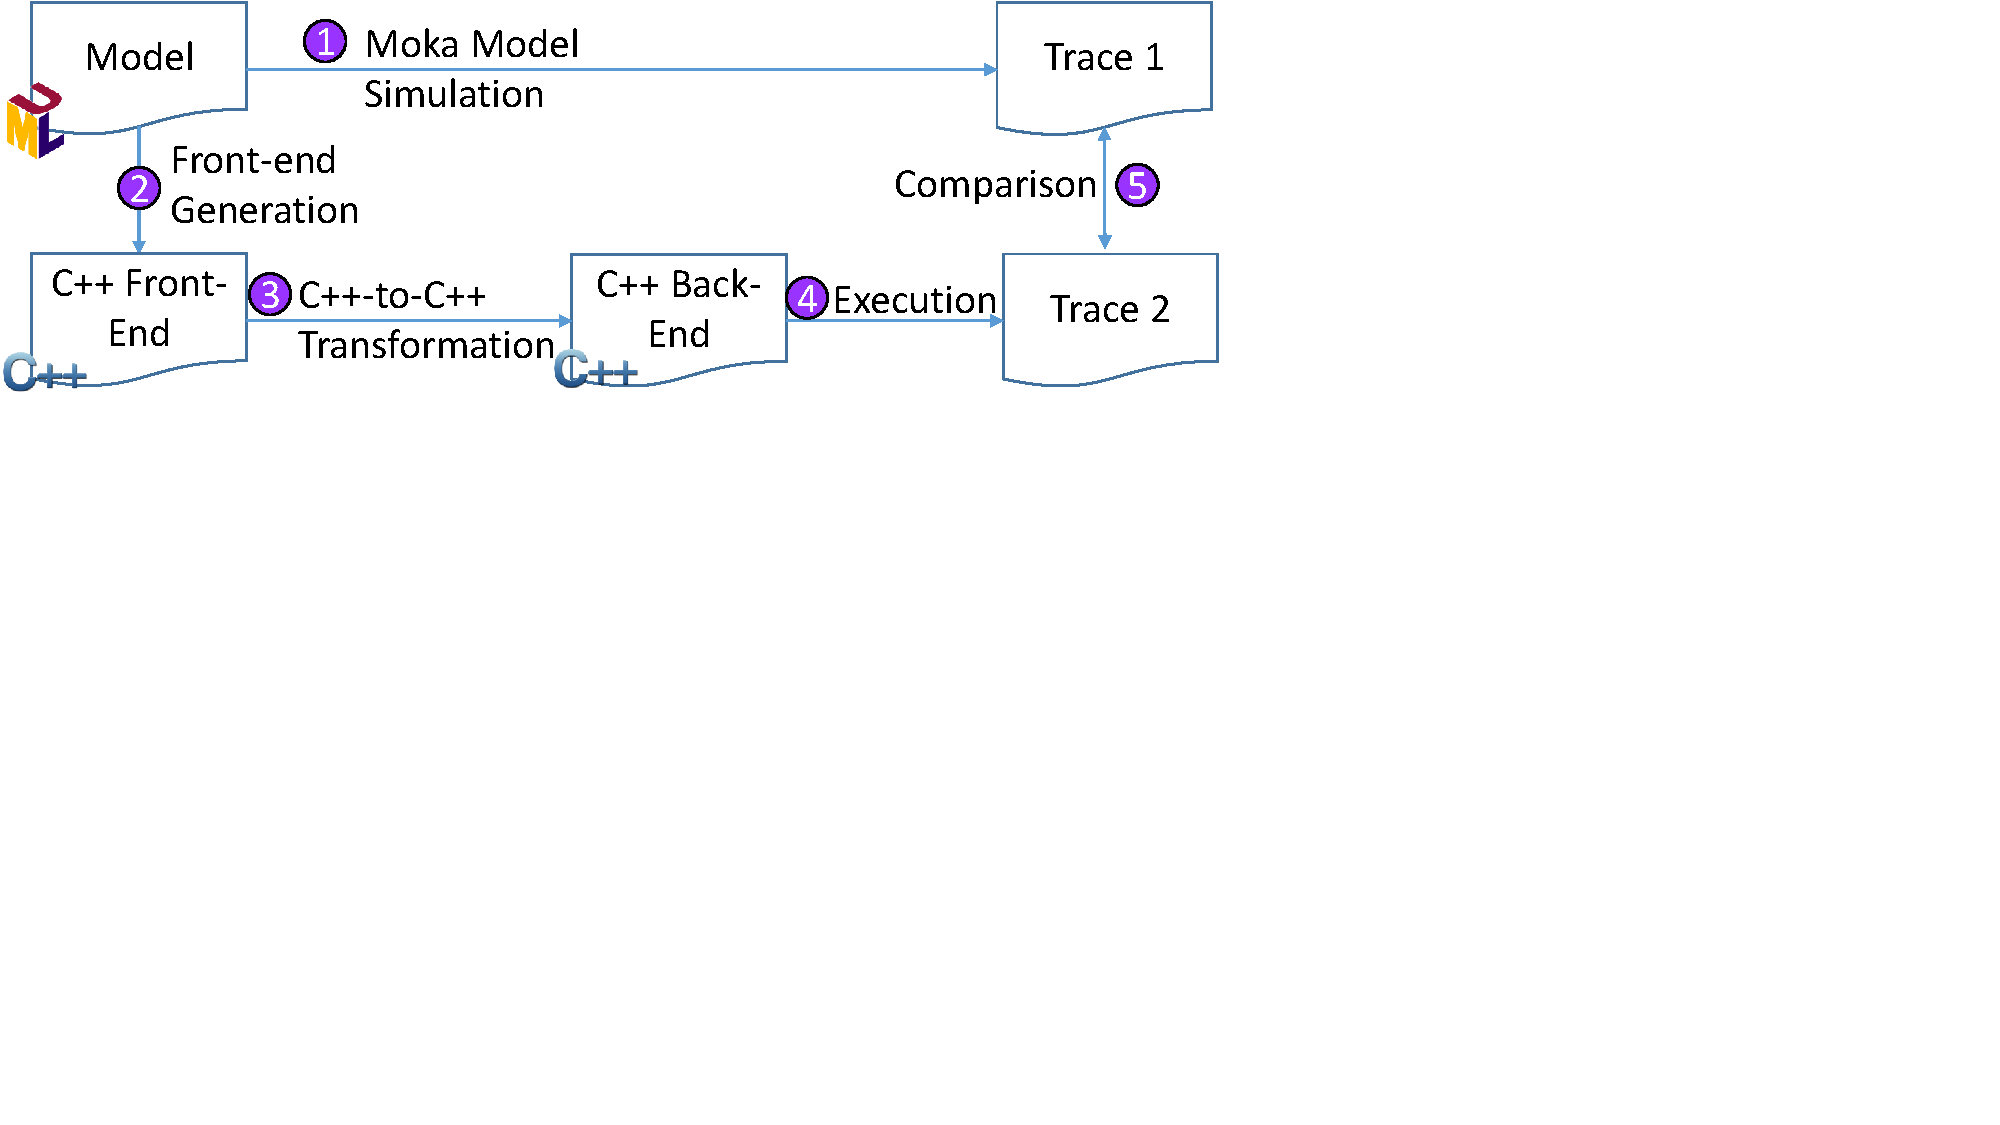
\includegraphics[clip, trim=0cm 12.0cm 12.7cm 0cm, width=\columnwidth]{figures/semanticconformance.pdf}
	\caption{Semantic conformance evaluation methodology} 
	\label{fig:semanticconformance}
\end{figure}		


\begin{table*}[]
	\centering
	\caption{Semantic-conformance test results (number of passed/total tests)}
	\label{table:semantic-test}
	\begin{tabular}{|l|l|l|l|l|l|l|l|l|l|l|l|l|l|}
		\hline
		Behavior & Choice & Deferred Events & Entering & Exiting & Entry & Exit & Event & Final & Fork & Join & Transition & Terminate & Others \\ \hline
		5/6&        3/3&         6/6        &    5/5      &    4/5     &  5/5     &   3/3   &    9/9    &   1/1    &   2/2   &   2/2   &      11/14      &    3/3       &    2/2    \\ \hline
	\end{tabular}
\end{table*}
\end{comment}


%\noindent
%\tb{Threats to validity:}
%Internal threat is that, all test cases of the PSSM test suite are contained in a single model file.
%However, the input to our experiments requires a test case per model file.
%Furthermore, operation behaviors, in PSSM, are defined by activities while our prototype defines behaviors as code blocks embedded into models.
%Therefore, we manually re-create these tests and convert activities into programming language code.

\subsection{Benchmarks}
\label{subsec:exp3}
In this section, we present the results obtained through the experiments on some efficiency aspects of back-end code to answer \tb{RQ3}. 
%Specifically, our research question related to memory consumption and runtime performance of generated code is stated as the following. 

%\noindent
%\tb{RQ3:} \ti{}



%\noindent
%\tb{Experimental dataset:} 
Two state machine examples are obtained by the preferred benchmark used by the Boost C++ libraries \cite{boost} in \cite{benchmark}. One simple example \cite{simpleexample} only consists of atomic states and the other \cite{compositeexample} both atomic and composite states. 

Code generation tools such as Sinelabore (which efficiently generates code for Magic Draw \cite{Magicdraw}, Enterprise Architect \cite{EA}) and QM \cite{qm}
%, which generate code from state machines
, and C++ libraries (Boost Statechart \cite{Statechart}, Meta State Machine (MSM) \cite{MSM}, C++ 14 MSM-Lite \cite{benchmark}, and functional programming like-EUML\cite{EUML}) are used for evaluation. 
%The tools are Sinelabore, which efficiently generates code from UML State Machines created by various modeling tools such as Magic Draw \cite{Magicdraw}, Enterprise Architect \cite{EA}, and QM \cite{QM}. 
%C++ libraries are Boost Statechart \cite{Statechart}, Meta State Machine (MSM) \cite{MSM}, MSM-Lite \cite{MSMLite}, and EUML \cite{euml}.

\noindent
\tb{Experimental procedures:} We use a Ubuntu virtual machine 64 bit (RAM, memory, Ghz??) hosted by a Windows 7 machine. 
For each tool and library, we created two applications corresponding to the two examples, generated C++ code and compiled it two modes: normal (N), by default GCC compiler, and optimal (O) with options -O2 -s. 
11 millions of events are generated and processed by the simple example and more than 4 millions for the composite example. 
%More than 4 millions of events are processed by the composite example. 
Processing time is measured for each case. 

\subsubsection{Speed} 
Fig. \ref{fig:boxplot} shows the event processing performance of the approaches.
%Table \ref{table-speed} shows the median of event processing time. 
In the normal compilation mode (N), Boost Statechart, MSM, MSMLite, EUML are quite slow and not displayed in the box-plot. 
Only Sinelabore and QM are performantly comparable with our approach. 
The table also shows that the optimization of GCC is significant. 
MSM and MSMLite run faster than Sinelabore and QM.   
%Boxplots in Fig. \ref{fig:boxplotsimple} and \ref{fig:boxplotcomposite} compare the performance of these approaches to that of our approach for the two examples, respectively. 
%In both of the simple and composite examples, 

Our approach processes faster around 40 milliseconds than the fastest approach within the scope of the experiment.
It is seen that, even without GCC optimizations, code generated by our approach significantly runs faster than that of EUML and QM with the optimizations. 
When compiled with the optimizations, our approach improves the event processing speed. 
Even, in case of composite, our approach does not produce any slowness compared to the simple example. 


% Please add the following required packages to your document preamble:
% \usepackage{multirow}
\begin{comment}
\begin{table*}[]
	\centering
	\caption{Event processing speed in ms}
\label{my-label}
\begin{tabular}{|l|l|l|l|l|l|l|l|l|l|l|l|l|l|l|l|l|}
	\hline
	\multicolumn{1}{|c|}{\multirow{2}{*}{Test}} & \multicolumn{2}{c|}{SC} & \multicolumn{2}{c|}{MSM} & \multicolumn{2}{c|}{MSM-Lite} & \multicolumn{2}{c|}{EUML} & \multicolumn{2}{c|}{Sinelabore} & \multicolumn{2}{c|}{QM} & \multicolumn{2}{l|}{Umple} & \multicolumn{2}{c|}{Our approach} \\ \cline{2-17} 
	\multicolumn{1}{|c|}{}                      & N           & O         & N            & O         & N              & O            & N            & O          & N               & O             & N          & O          & N            & O           & N                & O              \\ \hline
	Simple                                      & 13705,75    & 1658,1    & 5249,57      & 70,63     & 833,67         & 79,37        & 10867,93     & 109,97     & 141,03          & 79,93         & 285,9      & 229,27     & X            & X           & 106,87           & 25,37          \\ \hline
	Composite                                   & 5353,03     & 820,63    & 3546,1       & 46,73     & 516,87         & 65,17        & 4225,57      & 92,3       & 100,03          & 86,03         & 146,23     & 97,57      & X            & X           & 36,47            & 1,40           \\ \hline
\end{tabular}
\end{table*}
\end{comment}

\begin{comment}
\begin{table*}[]
	\centering
	\caption{Event processing speed in ms}
	\label{table-speed}
	\begin{tabular}{|l|l|l|l|l|l|l|l|l|l|l|l|l|l|l|l|l|}
		\hline
		\multicolumn{1}{|c|}{\multirow{2}{*}{Test}} & \multicolumn{2}{c|}{SC} & \multicolumn{2}{c|}{MSM} & \multicolumn{2}{c|}{MSM-Lite} & \multicolumn{2}{c|}{EUML} & \multicolumn{2}{c|}{Sinelabore} & \multicolumn{2}{c|}{QM} & \multicolumn{2}{l|}{Umple} & \multicolumn{2}{c|}{Our approach} \\ \cline{2-17} 
		\multicolumn{1}{|c|}{}                      & N           & O         & N            & O         & N              & O            & N            & O          & N               & O             & N          & O          & N            & O           & N                & O              \\ \hline
		Simple                                      & 13706    & 1658    & 5250      & 71     & 834         & 79        & 10868     & 110     & 141          & 80         & 286      & 229     & X            & X           & 107           & 25,4          \\ \hline
		Composite                                   & 5353     & 821    & 3546       & 47     & 517         & 65        & 4225,6      & 92       & 100          & 86         & 146     & 98      & X            & X           & 36,5            & 1,40           \\ \hline
	\end{tabular}
\end{table*}
\end{comment}


\begin{comment}
\begin{table*}[]
	\centering
	\caption{Event processing speed in ms}
	\label{table-speed}
	\begin{tabular}{|l|l|l|l|l|l|l|l|l|l|l|l|l|l|l|}
		\hline
		\multicolumn{1}{|c|}{\multirow{2}{*}{Test}} & \multicolumn{2}{c|}{SC} & \multicolumn{2}{c|}{MSM} & \multicolumn{2}{c|}{MSM-Lite} & \multicolumn{2}{c|}{EUML} & \multicolumn{2}{c|}{Sinelabore} & \multicolumn{2}{c|}{QM} & \multicolumn{2}{c|}{PSM} \\ \cline{2-15} 
		\multicolumn{1}{|c|}{}                      & N           & O         & N            & O         & N              & O            & N             & O         & N               & O             & N          & O          & N           & O          \\ \hline
		Simple                                      & 13706       & 1658      & 5250         & 71        & 834            & 79           & 10868         & 110       & 141             & 80            & 286        & 229        & 107         & 25,4       \\ \hline
		Composite                                   & 5353        & 821       & 3546         & 47        & 517            & 65           & 4225,6        & 92        & 100             & 86            & 146        & 98         & 36,5        & 1,40       \\ \hline
	\end{tabular}
\end{table*}
\end{coment}


\begin{comment}
\begin{figure}
	\centering
	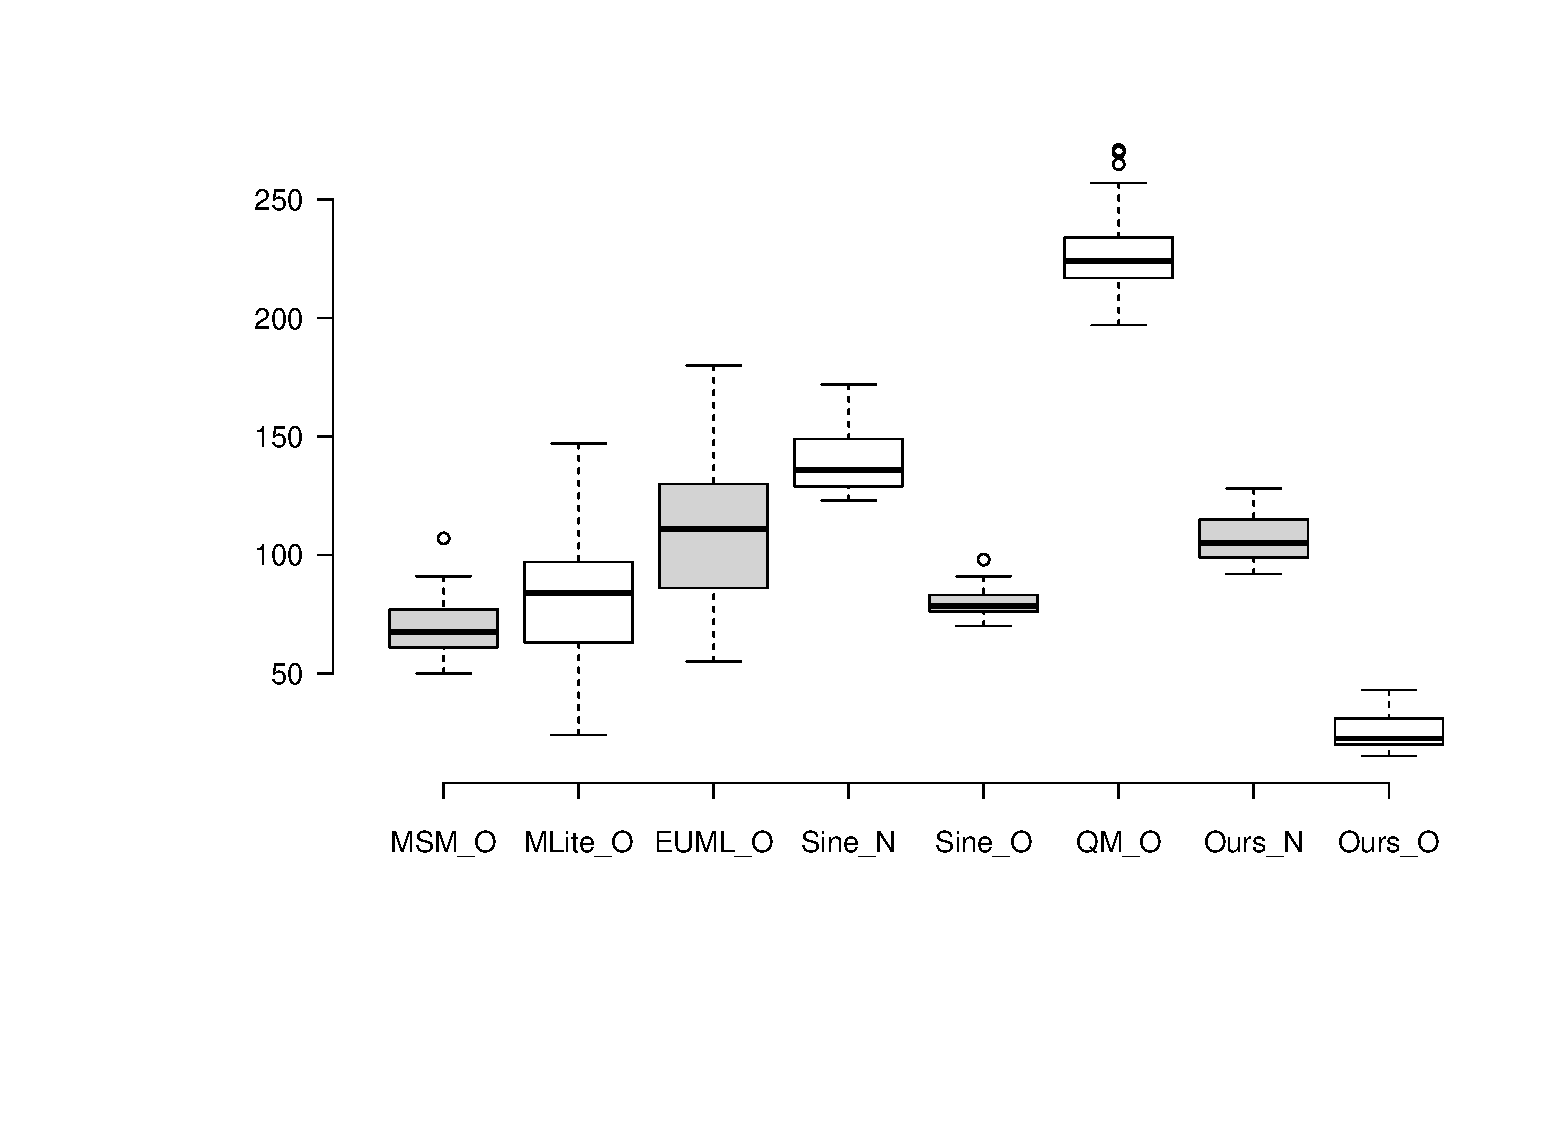
\includegraphics[clip, trim=4.2cm 4.6cm 1.7cm 2.3cm, width=\columnwidth]{figures/boxplotsimple.pdf}
	\caption{Event processing speed for the \ti{Simple} benchmark} 
	\label{fig:boxplotsimple}
\end{figure}

\begin{figure}
	\centering
	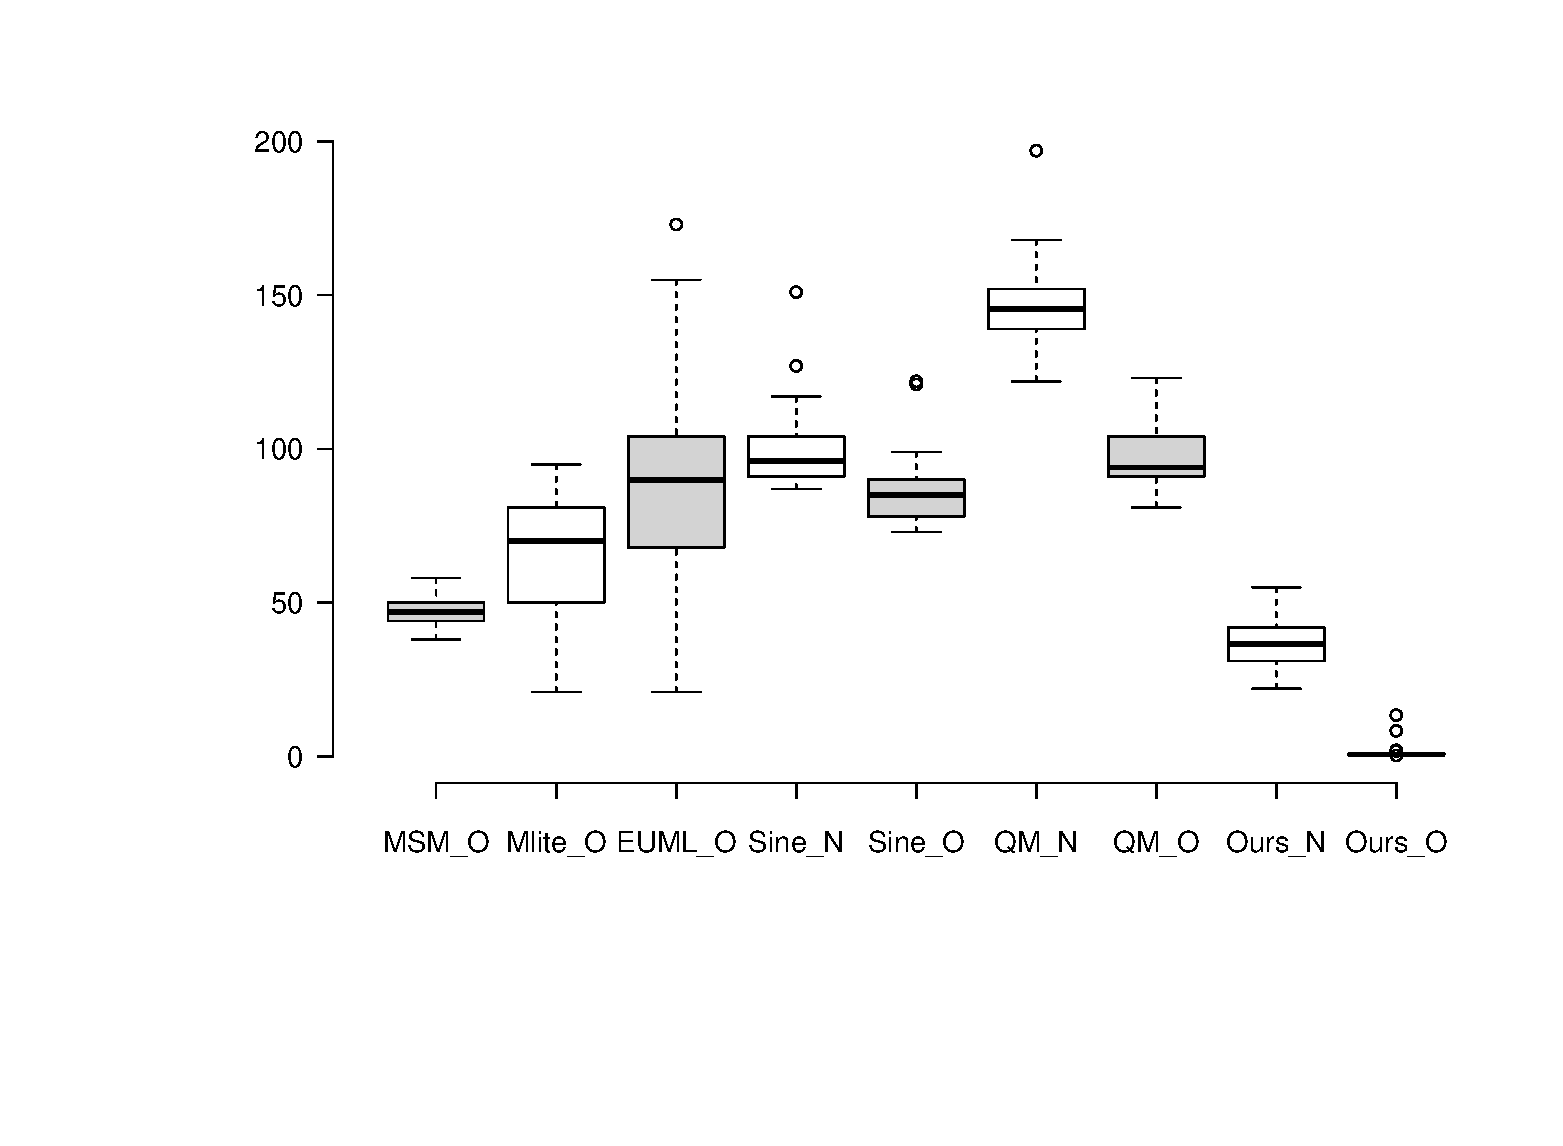
\includegraphics[clip, trim=4.2cm 4.6cm 1.7cm 1.8cm, width=\columnwidth]{figures/boxplotcomposite.pdf}
	\caption{Event processing speed for the \ti{Composite} benchmark} 
	\label{fig:boxplotcomposite}
\end{figure}
\end{comment}

\begin{figure}
	\centering
	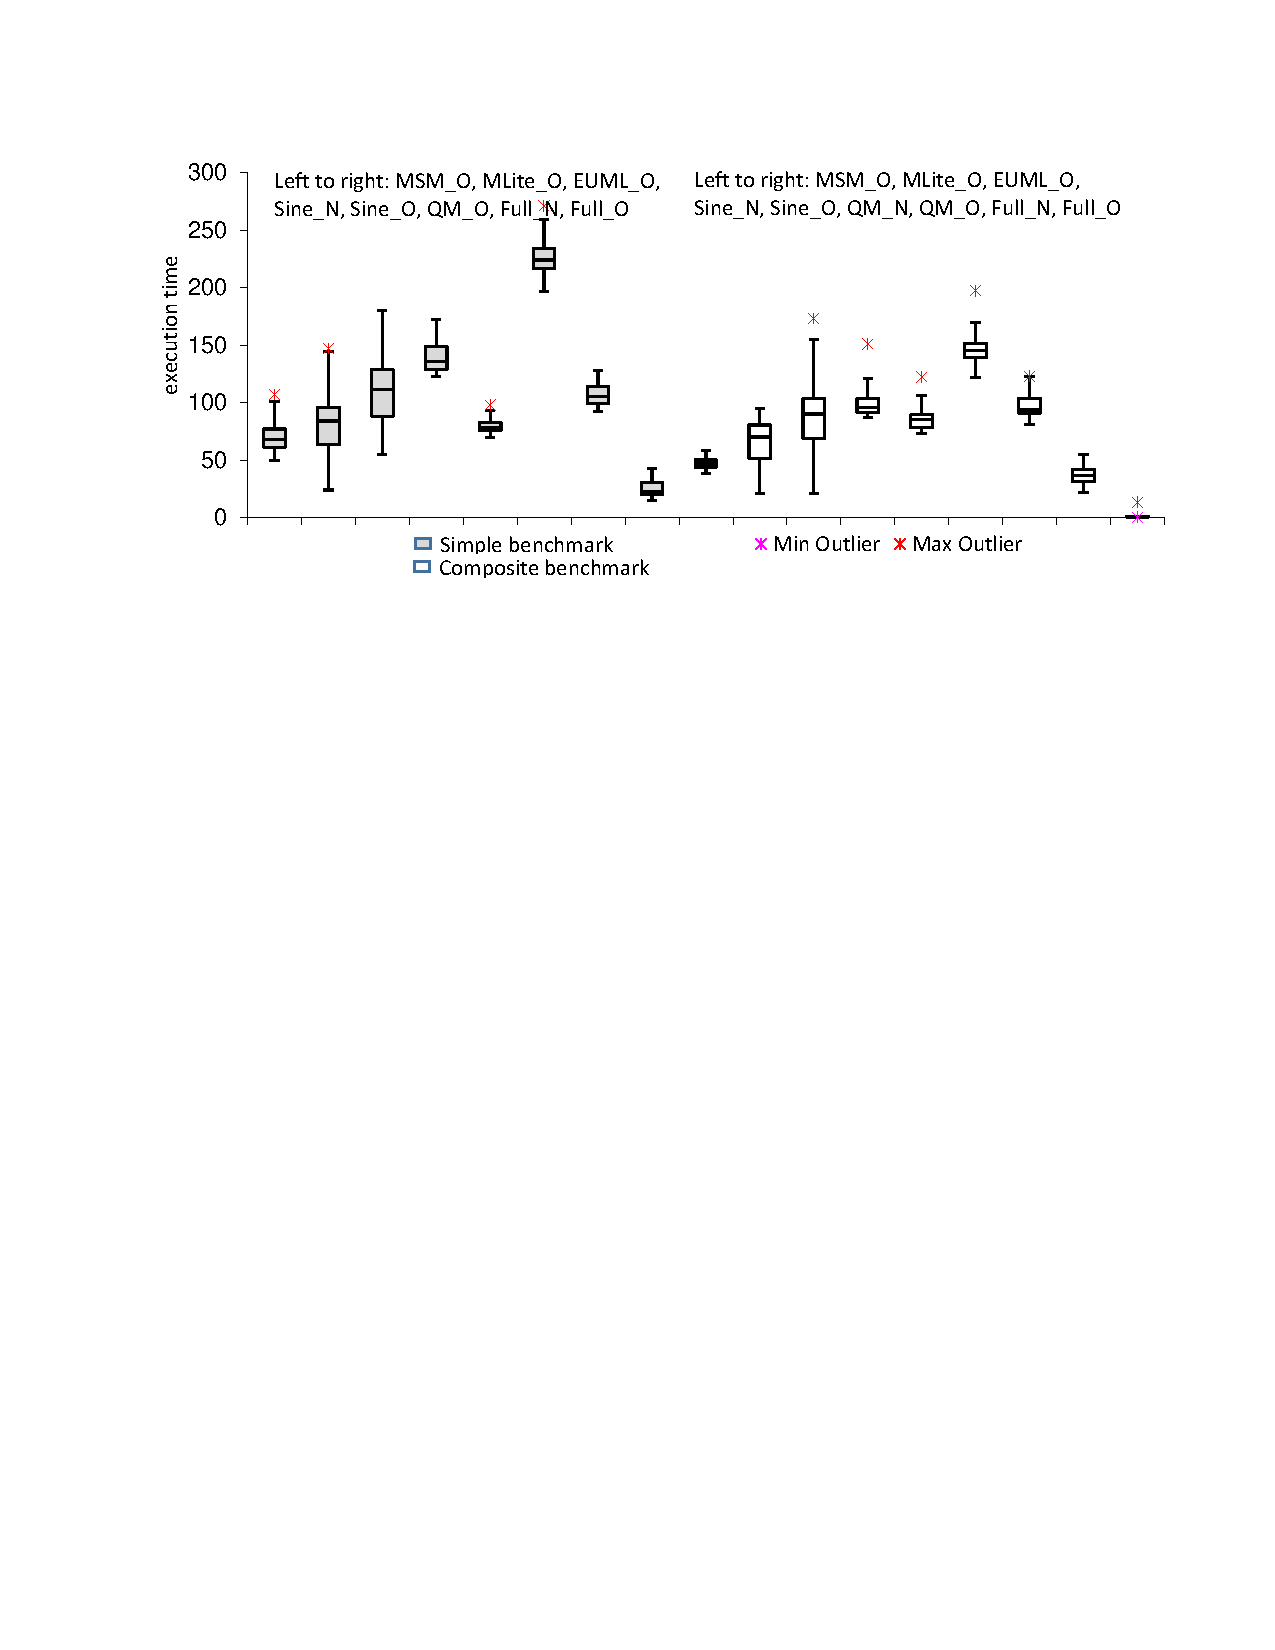
\includegraphics[clip, trim=2.8cm 18.0cm 1.7cm 2.5cm, width=\columnwidth]{experiments/box-plot-mine.pdf}
	\caption{Event processing speed for the benchmark} 
	\label{fig:boxplot}
\end{figure}

\subsubsection{Binary size and runtime memory consumption} 
Table \ref{table-size} shows the executable size for the examples compiled in two modes.
It is seen that, in GCC normal mode, Sinelabore generates the smallest executable size while our approach takes the second place.
When using the GCC optimization options, QM and our approach require less static memory than others. 

Considering runtime memory consumption, we use the Valgrind Massif profiler\cite{Massif} to measure memory usage. 
Table \ref{table:usage} shows the measurements for the composite example. 
Compared to others, code generated by our approach requires a slight overhead runtime memory usage (1KB).
This is predictable since the major part of the overhead is used for C++ multi-threading using POSIX Threads and resource control using POSIX Mutex and Condition. 
However, the overhead is small and acceptable (1KB). 


\begin{comment}
\begin{table*}[]
	\centering
	\caption{Executable size in Kb}
	\label{table-size}
	\begin{tabular}{|l|l|l|l|l|l|l|l|l|l|l|l|l|l|l|l|l|}
		\hline
		\multirow{2}{*}{Test} & \multicolumn{2}{c|}{SC} & \multicolumn{2}{c|}{MSM} & \multicolumn{2}{c|}{MSM-Lite} & \multicolumn{2}{c|}{EUML} & \multicolumn{2}{c|}{Sinelabore} & \multicolumn{2}{c|}{QM} & \multicolumn{2}{l|}{Umple} & \multicolumn{2}{c|}{Our approach} \\ \cline{2-17} 
		& N           & O         & N           & O          & N              & O            & N            & O          & N              & O              & N          & O          & N            & O           & N               & O               \\ \hline
		Simple                & 320      & 63,9     & 414,6      & 22,9      & 107,3         & 10,6        & 2339      & 67,9      & 16,5          & 10,6          & 22,6      & 10,5      &       X       &       X      & 21,5           & 10,6           \\ \hline
		Composite             & 435,8      & 84,4     & 837,4      & 31,1      & 159,2         & 10,9        & 4304,8      & 92,5      & 16,6          & 10,6          & 23,4      & 21,5      & X           & X          & 21,6           & 10,6           \\ \hline
	\end{tabular}
\end{table*}
\end{comment}

\begin{table*}[]
	\centering
	\caption{Executable size in Kb}
	\label{table-size}
	\begin{tabular}{|l|l|l|l|l|l|l|l|l|l|l|l|l|l|l|}
		\hline
		\multirow{2}{*}{Test} & \multicolumn{2}{c|}{SC} & \multicolumn{2}{c|}{MSM} & \multicolumn{2}{c|}{MSM-Lite} & \multicolumn{2}{c|}{EUML} & \multicolumn{2}{c|}{Sinelabore} & \multicolumn{2}{c|}{QM} & \multicolumn{2}{c|}{RAOES} \\ \cline{2-15} 
		& N           & O         & N           & O          & N              & O            & N            & O          & N              & O              & N          & O          & N           & O          \\ \hline
		Simple                & 320         & 63,9      & 414,6       & 22,9       & 107,3          & 10,6         & 2339         & 67,9       & 16,5           & 10,6           & 22,6       & 10,5       & 21,5        & 10,6       \\ \hline
		Composite             & 435,8       & 84,4      & 837,4       & 31,1       & 159,2          & 10,9         & 4304,8       & 92,5       & 16,6           & 10,6           & 23,4       & 21,5       & 21,6        & 10,6       \\ \hline
	\end{tabular}
\end{table*}

%\subsubsection{Runtime memory consumption}

\begin{table}[]
	\centering
	\caption{Runtime memory consumption in KB. Columns (1) to (7) are SC, MSM, MSM-Lite, EUML, Sinelabore, QM, and our approach, respectively.}
	\label{table:usage}
	\begin{tabular}{|l|l|l|l|l|l|l|l|l|}
		\hline
		Test      & (1)    & (2)  & (3) & (4) & \begin{tabular}[c]{@{}l@{}}(5)\end{tabular} & (6)    & \begin{tabular}[c]{@{}l@{}}(7)\end{tabular} \\ \hline
		Composite & 76.03 & 75.5 & 75.8  & 75.5 & 75.8                                                  & 75.7      & 76.5                                                   \\ \hline
	\end{tabular}
\end{table}


%\lipsum[1-6]